% ============================================================
%  Introduction — H&E to Sirius Red Virtual Staining Paper
%  Compile with: pdflatex + bibtex (or biblatex/biber)
%  NOTE: [TBC] markers denote citations needing author verification
% ============================================================
\section{Introduction}

\begin{figure*}[t!]
  \centering
  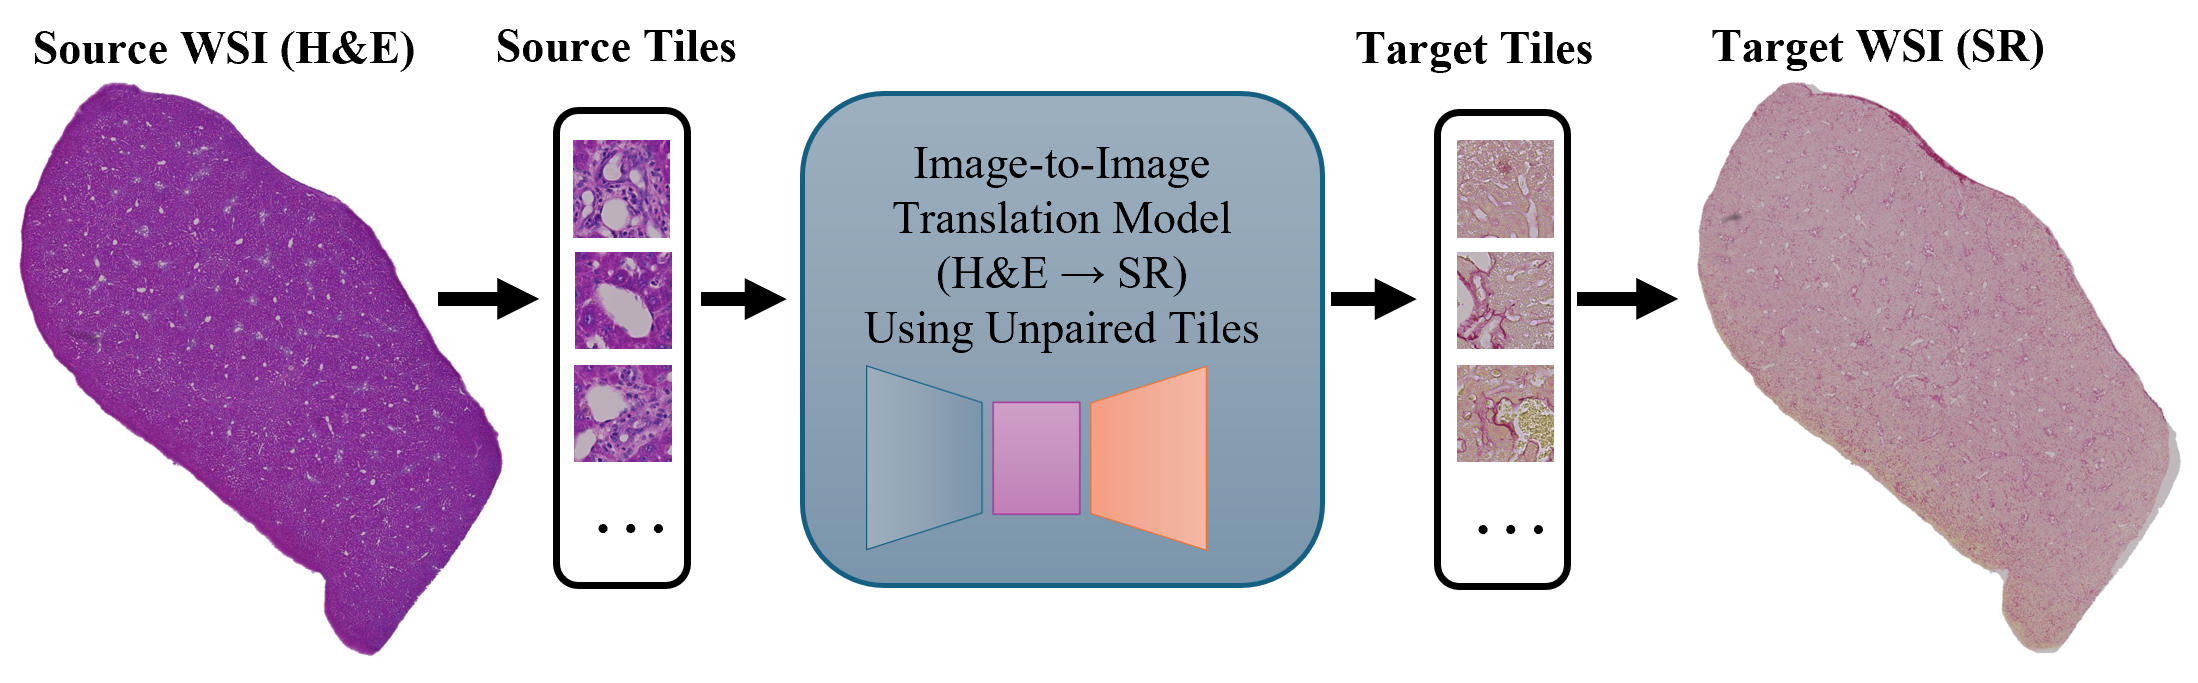
\includegraphics[width=0.92\linewidth]{images/translation.png}
  \caption{%
    Overview of the virtual H\&E~$\to$~SR staining pipeline studied in this work.
    A whole-slide image~(WSI) acquired with H\&E staining is decomposed into
    $256{\times}256$\,pixel tiles, which are passed through an unpaired
    image-to-image translation model to produce virtual Sirius Red tiles.
    The translated tiles are reassembled into a virtual SR WSI, from which
    collagen proportionate area~(CPA) can be quantified without consuming
    an additional tissue section.%
  }
  \label{fig:pipeline_overview}
\end{figure*}

Histopathology relies on a panel of stains that highlight different tissue components:
hematoxylin and eosin~(H\&E) shows overall tissue architecture, while specialised
stains target specific features such as collagen fibres, proliferating cells, or
receptor-expressing cells~\cite{lefkowitch2006special, krishna2013role}.
In clinical and preclinical practice, however, each additional stain requires a separate
tissue section. This consumes limited biopsy material~\cite{rivenson2020emerging, dehaan2021deep},
extends laboratory processing time~\cite{dehaan2021deep}, and introduces spatial
misalignment between stains because tissue deforms during sectioning and
mounting~\cite{gatenbee2023virtual, chen2022mvfstain}.
These costs grow with each marker: a full tissue characterisation panel may require four
or more serial sections from a single biopsy~\cite{clark2017immunohistochemistry},
limiting how much can be learnt from any given specimen.

These costs are especially limiting in liver pathology, where Sirius Red~(SR) binds
collagen with high specificity and serves as the gold-standard stain for measuring
collagen proportionate area~(CPA) and grading fibrosis, correlating more strongly with
serum fibrosis markers than Masson's trichrome~\cite{huang2013sirius}.

Virtual staining offers an attractive solution: it uses deep learning to predict a
target stain directly from an existing H\&E image (Figure~\ref{fig:pipeline_overview}).
By avoiding the need for additional sections, it conserves tissue, reduces turn-around
time, and enables retrospective analysis of H\&E
archives~\cite{rivenson2020emerging, latonen2024virtual}.
The field has advanced rapidly: supervised pixel-to-pixel models have been validated for
H\&E~$\to$~trichrome on large liver cohorts~\cite{kieffer2020largescale}, and a
prior-guided GAN has reached a Spearman correlation of $r_s{=}0.82$ between virtual and
real trichrome fibrosis scores~\cite{li2023unpaired}.
Yet supervised approaches require pixel-aligned image pairs from adjacent sections,
which is impractical at scale and introduces bias from tissue
deformation~\cite{aatresh2024virtual}.
\textit{Unsupervised} methods, which learn from unpaired image collections, are better
suited to this setting. However, to our knowledge, no prior work has systematically
compared them for H\&E~$\to$~SR translation in liver tissue; existing comparisons focus
almost entirely on H\&E~$\to$~IHC or skin staining~\cite{visgab2025, adib2024dual}.
Existing benchmarks also fix a single model scale and data budget, leaving open how
model capacity and training data jointly affect translation quality, an important
question because liver biopsy cohorts vary widely in size across clinical centres.

Beyond translation quality, ensemble variance provides an indirect check: where
independently trained members disagree, the unsupervised objective does not pin down a
unique answer for that input, an indicator of epistemic uncertainty that complements
task-specific evaluation. Epistemic uncertainty can be
estimated via MC~dropout or deep
ensembles~\cite{gal2016dropout, lakshminarayanan2017simple}, both applied to H\&E
classification and SR collagen segmentation~\cite{uncertainty_informed_hist2022,
liverfibrosis2025}, yet neither has been applied to unpaired image-to-image~(I2I) stain
translation. A
recent calibration study found MC~dropout poorly suited to unpaired
generation~\cite{trustworthy_i2i2025}, leaving deep ensembles as the more reliable
choice for this setting.

To address these open questions, this paper makes three contributions.

First, we conduct a full-factorial scaling study of six unsupervised I2I architectures
spanning GAN-based and diffusion-based families (CycleGAN~\cite{zhu2017unpaired},
UNIT~\cite{liu2017unsupervised}, MUNIT~\cite{huang2018multimodal},
DCLGAN~\cite{han2021dual}, UVCGAN~\cite{torbunov2022uvcgan}, and
CycleDiffusion~\cite{wu2022cyclediffusion}) at three generator capacities (${\sim}10$M, ${\sim}50$M, ${\sim}100$M
parameters) and three data fractions (25\%, 50\%, 100\%). Each of the 54 configurations
is evaluated using a task-specific CPA mean absolute error~(CPA~MAE), computed by
applying a frozen collagen segmentation model to real and virtual SR images, alongside
FID, LPIPS, and patch-SSIM.

Building on this study, we train deep ensembles of ten independently seeded models for
the best configuration per family, producing spatially resolved uncertainty maps and the
first systematic comparison of epistemic uncertainty across unsupervised stain-to-stain
architectures.

Finally, we release the whole-slide image dataset of paired H\&E and Sirius Red sections
from a mouse bile-duct ligation~(BDL) experiment~\cite{ghallab2025asbt}, the first open
resource for unsupervised H\&E~$\to$~SR translation in mouse liver tissue.
Together, these three contributions move unsupervised stain translation toward
reliable, uncertainty-aware evaluation.
% ============================================================
%  Bibliography entries specific to this section
%  (merge with references.bib; shared entries already in related_work.tex)
% ============================================================
%
% @article{Bataller2005,
%   author  = {Bataller, Ramon and Brenner, David A.},
%   title   = {Liver fibrosis},
%   journal = {Journal of Clinical Investigation},
%   volume  = {115},
%   number  = {2},
%   pages   = {209--218},
%   year    = {2005},
%   doi     = {10.1172/JCI24282}
% }
%
% @article{huang2013sirius,
%   author  = {Huang, Yi and de Boer, Wilhelmina B. and Adams, Leon A. and MacQuillan, Gerry and Bulsara, Max K. and Jeffrey, Gary P.},
%   title   = {Image analysis of liver collagen using sirius red is more accurate and correlates better with serum fibrosis markers than trichrome},
%   journal = {Liver International},
%   volume  = {33},
%   number  = {8},
%   pages   = {1249--1256},
%   year    = {2013},
%   doi     = {10.1111/liv.12184}
% }
%
% (All other entries shared with related_work.tex:
%  rivenson2020emerging, latonen2024virtual, kieffer2020largescale, li2023unpaired,
%  aatresh2024virtual, zhu2017unpaired, liu2017unsupervised, huang2018multimodal,
%  han2021dual, torbunov2022uvcgan, wu2022cyclediffusion, visgab2025, adib2024dual,
%  gal2016dropout, lakshminarayanan2017simple, uncertainty_informed_hist2022,
%  liverfibrosis2025, ugac2021, trustworthy_i2i2025)